\documentclass{article}
\usepackage[utf8]{inputenc}
\usepackage[T1]{fontenc}
\usepackage[export]{adjustbox}
\usepackage{mathtools,amsthm,amssymb,icomma,upgreek,xfrac,enumerate, bbm,titlesec,lmodern,polski,derivative,geometry,multicol,titling,graphicx,url,amsmath,caption,lipsum,float,longtable,booktabs}
\usepackage[table,xcdraw]{xcolor}
\usepackage[hidelinks,breaklinks,pdfusetitle,pdfdisplaydoctitle]{hyperref}
\setlength{\droptitle}{-1cm}
\mathtoolsset{showonlyrefs,mathic}
\title{Statystyka stosowana raport 1}
\author{Adam Wrzesiński, Joanna Kołaczek}
\date{30.04.2022}
\newtheoremstyle{break}
{\topsep}{\topsep}%
{\normalfont}{}%
{\bfseries}{}%
{\newline}{}%
\theoremstyle{break}
\newtheorem{zadanie}{Zadanie} 
\newtheorem*{rozwiazanie}{Rozwiązanie}

\titleformat*{\section}{\LARGE\bfseries}
\titleformat*{\subsection}{\Large\bfseries}
\titleformat*{\subsubsection}{\large\bfseries}
\titleformat*{\paragraph}{\large\bfseries}
\titleformat*{\subparagraph}{\large\bfseries}

%% KOMENDY:
\newcommand*{\e}{\mathrm{e}}
\newcommand{\hyline}[2]{%
	$#1$\> --\kern.5em #2 \\}


%% OPERATORY:
% `\diff` od „differential”, czyli odpowiednika słowa „różniczka” w języku
% angielskim.
\DeclareMathOperator{\diff}{d\!}
\newcommand{\indep}{\perp \!\!\! \perp}
\DeclareMathOperator{\EX}{\mathbb{E}}
\newcommand*{\E}{\mathrm{e}}



\begin{document}
	\maketitle
	\tableofcontents
	\clearpage
	\section{Wstęp}
	
	Niniejszy raport powstał na potrzeby realizacji laboratorium ze Statystyki Stosowanej, prowadzonych przez dr inż. Aleksandrę Grzesiek, do wykładu dr hab. inż. Krzysztofa Burneckiego. Będziemy analizować dane dotyczące długości ogonów myszołowów rdzawosternych (ang. red-tailed hawk). Dysponujemy próbą o wielkości 577 pobraną ze strony [1] . Na jej podstawie przedstawimy statystyki podzielone według miar położenia, rozproszenia, asymetrii oraz spłaszczenia. Na koniec pierwszego rozdziału zebrane wielkości przedstawimy w formie tabeli.  W drugiej części raportu zwizualizjemy dane za pomocą histogramu oraz wykresu pudełkowego. Wyznaczymy ponadto dystrybuantę empiryczną analizowanej próby. Na koniec wyniki badań omówimy w podsumowaniu. Życzymy Czytelnikowi miłej lektury.
	
	\section{Poznane statystyki}
	\subsection{Miary położenia}
	
	Miary położenia określają położenie pojedynczej wartości w stosunku do innych wartości w próbie. 
	
	\subsubsection{Średnia arytmetyczna}
	$$\overline{x}=\frac{1}{n}\sum\limits_{i=1}^{n}x_i$$
	Jest to suma wszystkich wartości z próby, podzielona przez ich ilość. Chociaż średnia arytmetyczna jest często używana do określania tendencji centralnej, nie jest to tzw statystka odpornościowa, co oznacza, że duży wpływ na nią mają wartości odstające. W przypadku rozkładów skośnych, takich jak np rozkład dochodów, w którym dochody kilku osób są znacznie wyższe niż dochody większości, średnia arytmetyczna może nie pokrywać się z naszym pojęciem "środka", dlatego lepiej można go określić z pomocą innych statystyk.\\
	Dla naszych danych średnia aryrmetyczna wyniosła: \textbf{222,149}
	\subsubsection{Średnia harmoniczna}
	$$\overline{x}_h=\frac{n}{\sum\limits_{i=1}^{n}\frac{1}{x_i}}$$
	Jest to liczba obserwacji podzielona przez sumę odwrotności wartości z próby. Często wykorzystuje się ją do obliczania średniej współczynników lub wskaźników lub gdy wartości danych są wyrażone w jednostkach w postaci względnej. Niejako wyrównuje ona wagę każdego punktu danych, na przykład średnia arytmetyczna przypisuje dużą wagę dużym zbiorom danych, podczas gdy średnia harmoniczna nadaje mniejszą wagę mniejszym zbiorom danych. (?) \\
	Dla naszych danych średnia harmoniczna wyniosła: \textbf{221.085}
	\subsubsection{Średnia geometryczna}
	$$\overline{x}_g=\sqrt{\prod\limits_{i=1}^{n}x_i}$$
	Jest to pierwiastek stopnia $n$ z iloczynu $n$ wartości próby. Średnia geometryczna jest często stosowana w przypadku zbioru liczb które mają charakter wykładniczy, np. zbioru danych dotyczących wzrostu: wartości populacji ludzkiej lub stóp procentowych inwestycji finansowych w czasie.
	\subsubsection{Średnia ucinana}
	$$\overline{x}_u=\frac{1}{n-2k}\sum\limits_{i=k+1}^{n-k}x_i$$
	Liczy się ją tak jak średnią arytmetyczną, jednak odrzuca się określony procent wartości skrajnych. Dzięki temu jest to estymator wrażliwy na wartości odstające - w przeciwieństwie do średniej arytmetycznej jest to prosty przykład statystyki odpornościowej. Używana chociażby przy ocenianiu przez sędziów w zawodach. Średnia obcięta wykorzystuje więcej informacji z rozkładu lub próby niż mediana, ale o ile rozkład podstawowy nie jest symetryczny, jest mało prawdopodobne, aby średnia obcięta z próby dała bezstronny estymator zarówno średniej, jak i mediany.
	\subsubsection{Średnia Winsorowska}
	$$\overline{x}_w=\frac{1}{n}[(k+1)x_{k+1}\sum\limits_{i=k+2}^{n-k-1}x_i +(k+1)x_{n-k}]$$
	Liczy się ją podobnie jak średnią ucinaną, jednak zamiast pozbywać się wartości skrajnych, zamienia się je na odpowiednio minimum i maksimum z pozostałych wartości. Ma ona również podobne własności co średnia ucinana, stosowana jest najczęściej w sytuacjach kiedy nie jesteśmy pewni co do prawdziwości, dokładności wartości skrajnych.
	\subsubsection{Kwantyle}
	Kwantyle dzielą uporządkowaną próbę na mniejsze grupy o równej ilości elementów. Najbardziej "znanym" kwantylem jest mediana, wartość środkowa, powyżej i poniżej niej znajduje się 50\% obserwacji. Dobrze się sprawdza gdy chcemy porównać zarobki ale znajduje też zastosowanie w grafice komputerowej, gdzie przydaje się przy odszumianiu. Kwartyle, które wskazują na dolne i górne 25\% również często pojawiają się przy porównywaniu wynagrodzeń.
	\paragraph{Mediana}
	$$x_{med}=
	\begin{cases}
		x, &  \text{gdy $n$ jest nieparzyste }\\
		\frac{1}{2}(x_{\frac{n}{2}}+x_{\frac{n}{2}+1}), &  \text{gdy $n$ jest parzyste}\\
	\end{cases}$$
	\paragraph{Kwartyle}
	\begin{itemize}
		\item drugi kwartyl ($Q2$) to mediana
		\item pierwszy kwartyl ($Q1$) to mediana grupy obserwacji mniejszych od $Q2$
		\item drugi kwartyl ($Q3$) to mediana grupy obserwacji większych od $Q2$
	\end{itemize}
	
	\subsection{Miary rozproszenia}
	
	Miary rozproszenia pozwalają określić zróżnicowanie wartości danej cechy wokół wartości centralnych (np. mediany, średniej).  Wskazują one, czy wyniki są zbliżone do wartości centralnej, czy też są znaczne różnice między poszczególnymi wynikami. Jeśli rozproszenie jest duże to wyliczona wartość centralna najczęściej niewiele nam powie o badanej grupie, jeśli wynik jest natomiast mały, to oznacza, że średnia lub mediana dobrze reprezentują wszystkie jednostki.
	
	\subsubsection{Rozstęp}
	$$R=x_n-x_1$$
	Jest to najprostsza miara rozproszenia - różnica między największą a najmniejszą zaobserwowaną wartością z próby. 
	\subsubsection{IQR (rozstęp międzykwartylowy)}
	$$IQR=Q3-Q1$$
	Jest to miara rozrzutu zmiennej, podobna do odchylenia standardowego, jednak bardziej odporna na elementy odstające. Wyznaczamy go jako różnicę między trzecim a pierwszym kwartylem.
	\subsubsection{Wariancja z próby}
	$$S^2=\frac{1}{n-1}\sum\limits_{i=1}^{n}(x_i - \overline{x})^2$$
	Wariancja to średnia arytmetyczna kwadratów odchyleń poszczególnych wartości zbioru i cechy od wartości oczekiwanej (przypadek obciążony).  Informuje nas, jak bardzo zróżnicowany jest zbiór pod kątem koncentracji wokół średniej bądź też rozproszenia - im bliżej zera, tym mniej zróżnicowane wartości w próbie. Jeżeli chcemy uzyskać wariancję nieobciążoną, w mianowniku musimy zamienić $n$ na $n-1$.
	\subsubsection{Odchylenie standardowe}
	
	$$S=\sqrt{S^2}$$
	
	Odchylenie standardowe to pierwiastek z wariancji z próby. Pokazuje rozrzut danych wokół średniej.
	
	\subsubsection{Współczynnik zmienności}
	$$V=\frac{S}{\overline{x}} \quad (\cdot 100\%)$$
	
	Wartość współczynnika zmienności wyznacza zróżnicowanie cechy i świadczy o niejednorodności badanej próby. Im mniejsza wartość, tym mniejsza zmienność cechy. Współczynnik zmienności jest ilorazem (wynikiem dzielenia) odchylenia standardowego cechy oraz jej średniej arytmetycznej.
	
	\subsection{Miary asymetrii}
	\subsubsection{Współczynnik skośności (asymetrii)}
	
	$$\alpha =\frac{n}{(n-1)(n-2)}\sum\limits_{i=1}^{n}(\frac{x_i-\overline{x}}{S})^3$$
	$$\alpha_1 =\frac{\frac{1}{n}\sum\limits_{i=1}^{n}(x_i-\overline{x})^3}{(\frac{1}{n}\sum\limits_{i=1}^{n}(x_i-\overline{x})^2)^{\frac{3}{2}}}$$
	
	Współczynnik asymetrii służy do badania kształtu rozkładu próby. Jeżeli jego wartość jest ujemna, to grzbiet rozkładu znajduje się po lewej stronie od średniej (lewostronna skośność). W przeciwnym wypadku mówimy o prawostronnej skośności. 
	
	\subsection{Miary spłaszczenia (koncentracji)}
	
	Miary koncentracji, tak jak nazwa wskazuje, mówi o koncentracji rozkładu próby wokół jej średniej.
	
	\subsubsection{Kurtoza}
	$$K_1 =\frac{\frac{1}{n}\sum\limits_{i=1}^{n}(x_i-\overline{x})^4}{(\frac{1}{n}\sum\limits_{i=1}^{n}(x_i-\overline{x})^2)^2}$$
	$$K=\frac{n-1}{(n-2)(n-3)}((n+1)K_1-3(n+1))+3$$
	
	Kurtoza jest miarą ilości wartości odstających w próbie. Dla rozkładu normalnego (w naszym przypadku) wynosi 3. Im mniejsza jej wartość, tym bardziej dane z próby są skupione wokół średniej.
	
	\subsection{Tabela}
	\begin{longtable}[c]{| c | c |}
		\hline
		\multicolumn{2}{|l|}{\cellcolor[HTML]{DBDBDB}Miary położenia}    \\ \hline
		\multicolumn{1}{|l|}{średnia arytmetyczna}          & 222.149    \\ \hline
		\multicolumn{1}{|l|}{średnia harmoniczna}           & 221.085    \\ \hline
		\multicolumn{1}{|l|}{średnia geometryczna}          & 221.643    \\ \hline
		\multicolumn{1}{|l|}{średnia ucinana}               & 222.104    \\ \hline
		\multicolumn{1}{|l|}{średnia Winsorowska}           & 222.182    \\ \hline
		\multicolumn{1}{|l|}{mediana Q2}                    & 214        \\ \hline
		\multicolumn{1}{|l|}{Q1}                            & 221        \\ \hline
		\multicolumn{1}{|l|}{Q3}                            & 230        \\ \hline
		\multicolumn{2}{|l|}{\cellcolor[HTML]{DBDBDB}Miary rozproszenia} \\ \hline
		\multicolumn{1}{|l|}{rozstęp}                       & 166        \\ \hline
		\multicolumn{1}{|l|}{IQR}                           & 16         \\ \hline
		\multicolumn{1}{|l|}{wariancja nieobciążona}        & 210.568    \\ \hline
		\multicolumn{1}{|l|}{wariancja obciążona}           & 210.203    \\ \hline
		\multicolumn{1}{|l|}{odchylenie standardowe}        & 14.511     \\ \hline
		\multicolumn{1}{|l|}{współczynnik zmienności}       & 6.532      \\ \hline
		\multicolumn{2}{|l|}{\cellcolor[HTML]{DBDBDB}Miary asymetrii}    \\ \hline
		\multicolumn{1}{|l|}{współczynnik skośności I}      & XD          \\ \hline
		\multicolumn{1}{|l|}{współczynnik skośności II}     & -0.848     \\ \hline
		\multicolumn{2}{|l|}{\cellcolor[HTML]{DBDBDB}Miary spłaszczenia} \\ \hline
		\multicolumn{1}{|l|}{Kurtoza}                       & 8.407      \\ \hline
	\end{longtable}
	
	\section{Wizualizacja}
	\subsection{Histogram}
	\begin{figure}[H]
		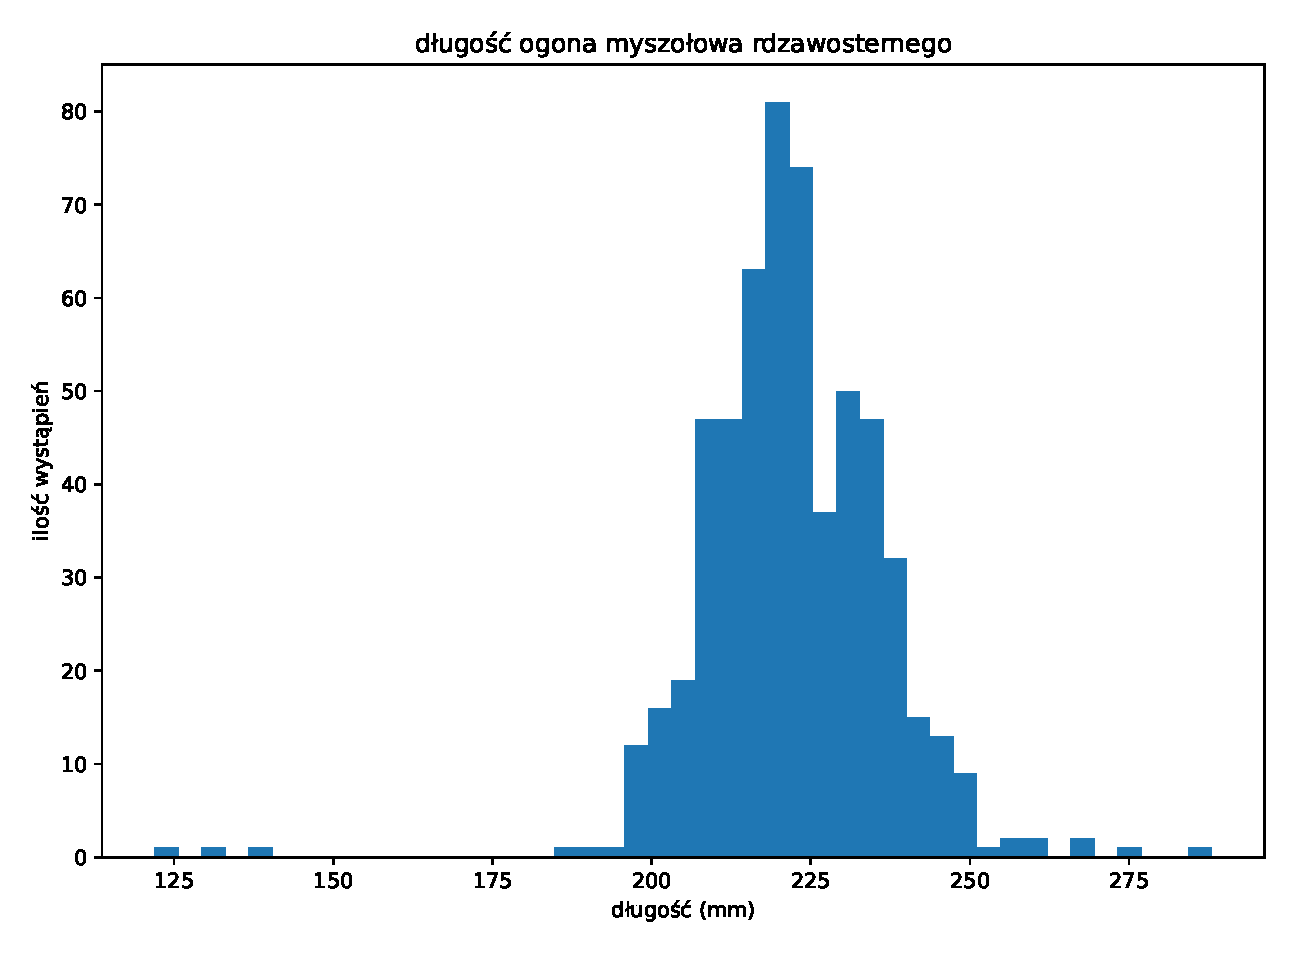
\includegraphics[scale=0.75]{HISTOGRAM.eps}
	\end{figure}
	\subsection{Boxplot}
	\begin{figure}[H]
		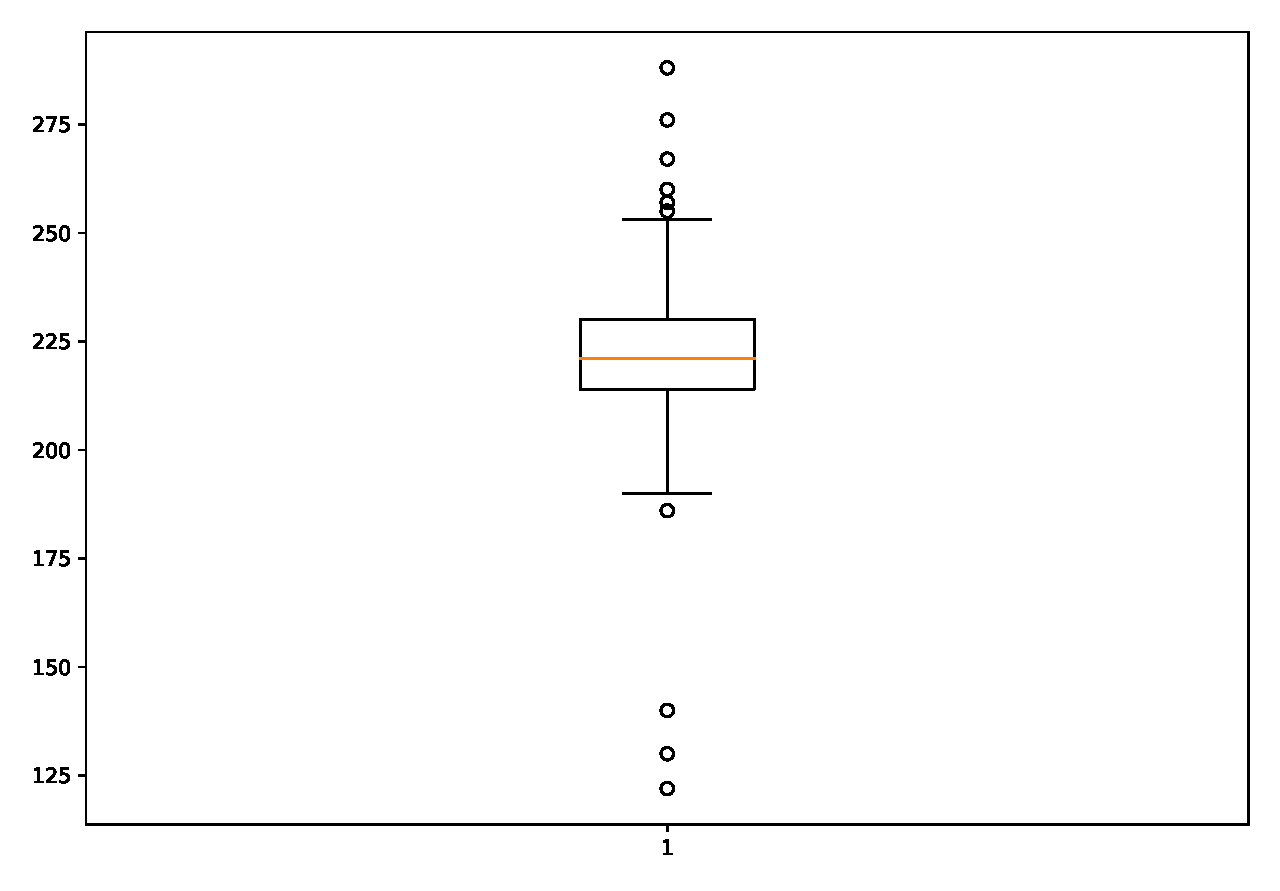
\includegraphics[scale=0.75]{BOXPLOT.eps}
	\end{figure}
	\subsection{Dystrybuanta empiryczna}
	\begin{figure}[H]
		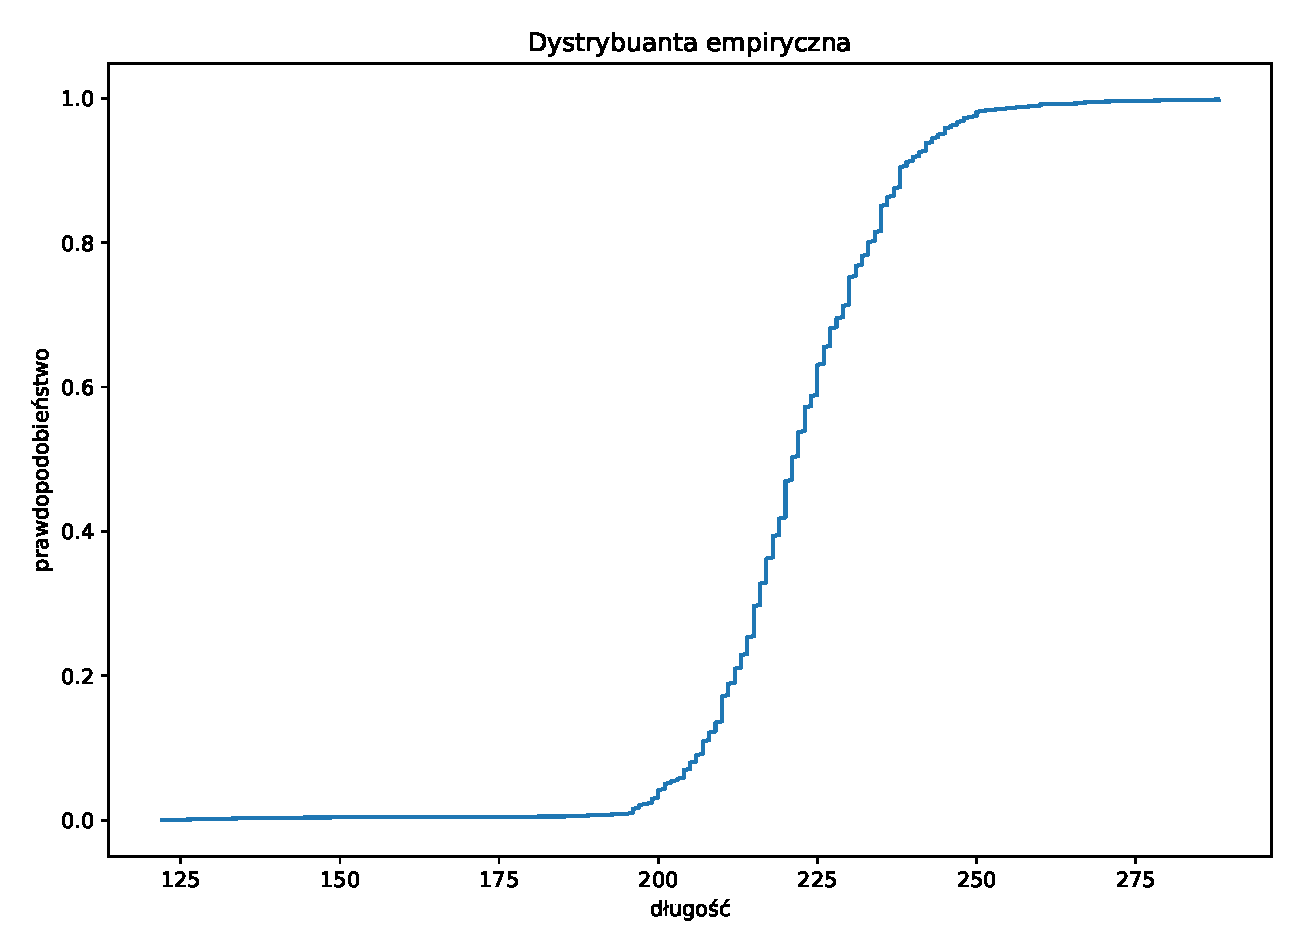
\includegraphics[scale=0.75]{DYSTRYBUANTA.eps}
	\end{figure}
	
	\section{Podsumowanie}
	
	
\end{document}